\section{Koalition}
\subsection{Overview}
%What is Koalition (as an LP and cryptocurrency)
%How does Koalition work wrt to points exchange
%to price stability
%For marketing, etc.
Koalition is a blockchain-based, decentralized loyalty program that aims to consolidate the myriad of existing and future loyalty programs into a single, vast interconnected and interoperable network. The individual LPs in the Koalition network are connected via a rewards-based unicurrency called \textit{KOA}, a price-stable cryptocurrency that enables frictionless exchange and redemption of rewards across the network. KOA boasts utility as well as usability as a stable coin, growing the crypto-economy as a liquid asset that users are more willing to use than typically deflationary cryptocurrencies. Consumers will not only be able to use KOA to pay for products and services across the Koalition network, they will also be able to exchange KOA freely among themselves and other entities on the network. This will enable a rich rewards-based economy that unlocks the value of brand loyalty.
%
\begin{figure}[h] % use "t!" to force the float to start the float at top of page
    \centering
        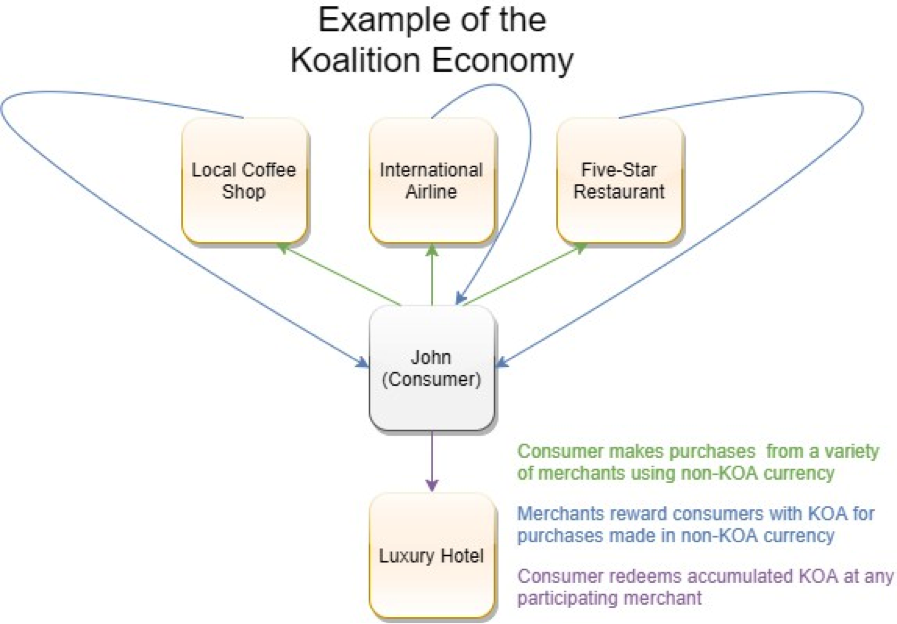
\includegraphics[keepaspectratio, width=0.7\textwidth]{images/KOAeconomy.png}
    \caption{The Koalition Economy} \label{fig:KOAeconomy}
\end{figure}

A paradigm shift in consumer behavioral and attitudinal loyalty has begun. Traditional stand-alone and coalition LPs have undoubtedly changed the dynamics of merchant competition and perpetuated the importance of relationship marketing. Koalition aims to satisfy customer demand through its vast network of merchants while maintaining integrity as a marketing tool for businesses by influencing customer buying behavior and perceptions through data analytics. Merchants now have the opportunity to embrace a disruptive technology that is bound to shake up the traditional LP economy. The following sections will discuss the intricacies of the Koalition protocol, specifically how it works, its limitations, and how it is bound to disrupt the loyalty programs space.
%
\begin{figure}[h]% use "t!" to force the float to start the float at top of page
	\centering
	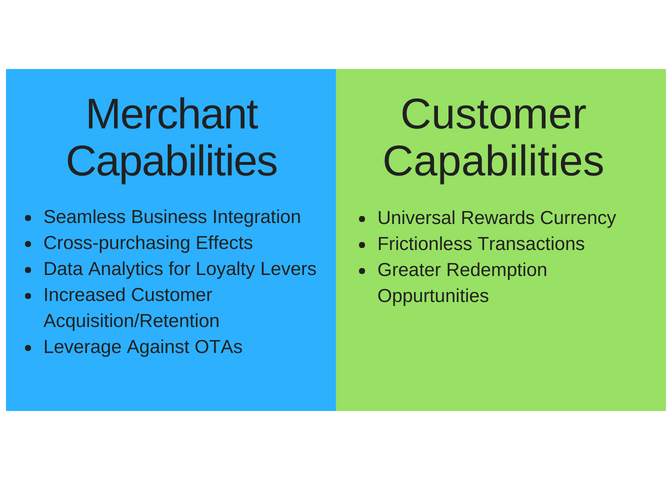
\includegraphics[keepaspectratio, width=0.6\textwidth]{images/KoaCapes.png} \\
\end{figure}
%
\subsection{Merchant Capabilities}

\subsubsection{Seamless Business Integration}
The Koalition loyalty program caters to the needs of all businesses selling products or services. From small local businesses to international corporations, each gain access to a network enhanced by blockchain technology. Small businesses gain access to a powerful marketing platform, opening their doors to a vast new customer acquisition and retention tool. Typically, small businesses do not have the infrastructure to build and support a robust LP. However, Koalition enables small businesses to integrate with current fiat payment options and will run effortlessly through autonomous contract execution. Furthermore, adopting cryptocurrencies as a means of payment eliminates large credit card transaction fees and delayed receipt of payments, which at times can be pivotal for small businesses.

For larger businesses, existing loyalty programs cannot be easily terminated from a marketing relationship perspective. Termination may be costly and negatively affect a company's image. Fundamentally, customer relationship management as a corporate strategy creates high exit barriers \cite{Rehnen16}. Therefore, Koalition offers the flexibility of two different adoption options that cater to operational risk tolerance and perceived practicality of implementation.  


\begin{enumerate}
\item \textbf{Option 1: ``Koexist" with existing LPs} \\
Merchants can choose to keep their existing LP while offering consumers the option to pay for goods and services/receive rewards in KOA or the merchant's native rewards currency. This non-invasive approach caters to businesses that have an existing LP that either wish to use both LPs indefinitely or are engineering a risk-averse exit strategy to their current LP.

\item \textbf{Option 2: Full Adoption of the Koalition Rewards Protocol} \\
Full adoption maximizes user utility for both merchants and consumers. Merchants who elect this option will replace all of the existing points in their current rewards program with KOA. The merchant must then choose how its customers who hold the native points can convert these to KOA (eg. convert cash value of native points to KOAs). Merchants who choose to fully adopt the Koalition Rewards Protocol will leverage the full extent of blockchain technology in the rewards economy. First, merchants will be fully integrated in a cooperative network where noncompetitive industries gain from each other. Second, liabilities akin to unredeemed rewards points become negligible as revenue is immediately realized.
\end{enumerate}

Streamlined onboarding of new partners perpetuates network effects. Koalition introduces an avenue for businesses of any size to partner with one another on one rewards network thus providing consumers with a convenient LP and introducing a paramount marketing opportunity to merchants. 

\subsubsection{Cross-purchasing Effects}

\textbf{Network Effects} \\
It has already been established that merchants have more to gain from a coalition LP than a stand-alone one. Liabilities are split and marketing opportunities increase as a result of LP partnerships. Koalition brings this concept to the next level with a universal LP giving merchants a superior marketing platform with virtually no liabilities (since KOA represents a real cash value) and consumers have a fungible rewards currency they can use across multiple industries. The analysis in Section \ref{sec:analysis} shows that existing merchants on the Koalition network benefit from the addition of new merchants since cross-purchasing between merchants increase. The effect here is two fold: As more consumers join the network, merchants enjoy opportunities for more data flow, customer acquisition/retention, and ultimately profits. As more merchants join the network, consumers enjoy a wider array of redemption options and purchasing power. Therefore, as the network grows, the more non-participating merchants and consumers are incentivized to join the network. 
%
\begin{figure}[h]
	\centering
	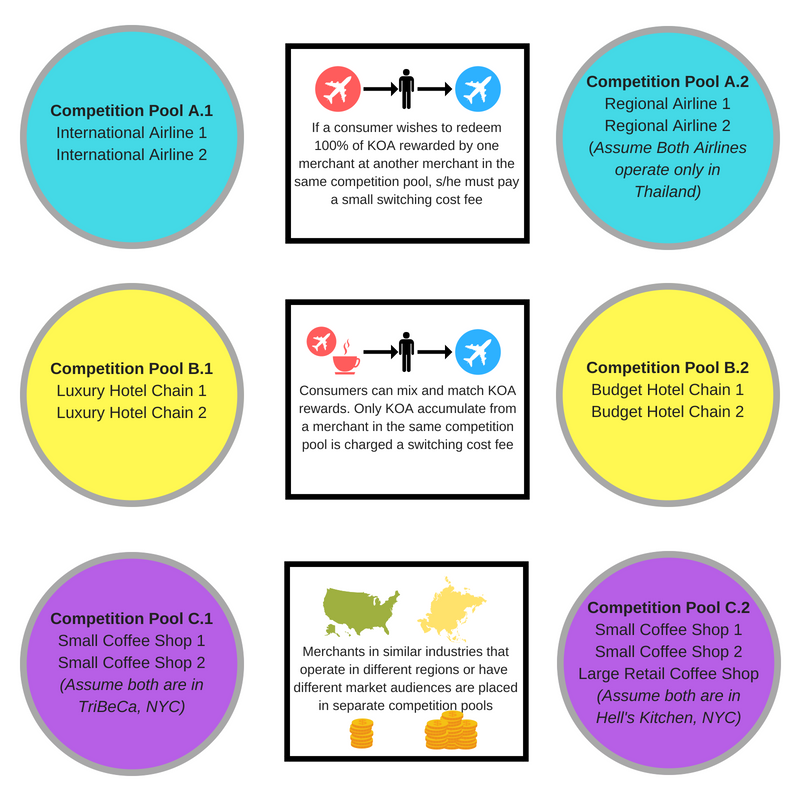
\includegraphics[keepaspectratio,width=.8\textwidth]{images/CompetitionPools.png}
	\caption{Competition Pools in the Koalition Network} \label{fig:competitionpool}
\end{figure}

\noindent \textbf{Equal-level Partnership and Switching Costs} \\
The Koalition loyalty program is based on an equal-level partnership model, leveraging network effects and encouraging cross-purchasing. In this model, KOA is redeemable across all merchants on the Koalition network. While it is freely redeemable between complementary merchants, a switching cost is applied between directly competing merchants. These directly competing merchants are placed in so called \textit{competition pools}. For example, consumers who accumulate points from International Airline 1 will be unable to redeem these points from International Airline 2 at full buying power if these two airlines are in the same competition pool. The fee percentage will be a predetermined fixed rate. Competition Pools are determined based on industry type, size of business, and operating locations. For example, two major airlines in the United States similar in market capitalization may be put in the same competition pool, but two non-chain coffee shops operating in different cities would not.

	
Furthermore, some merchants may be in the same industry, but are non-competitive amongst one another because they cater to customers in different economic backgrounds. A luxury hotel chain and a budget hotel chain would be placed in separate Competition Pools because they are not directly competitive so a consumer can have $100\%$ buying power between a luxury hotel and a budget hotel. 

Figure \ref{fig:competitionpool} above demonstrates how a consumer can use his/her KOAs that (s)he accumulates from a specific merchant. Consumers have $100\%$ buying power when redeeming KOAs at noncompetitive merchants. However, if a consumer accumulates points from one merchant and wishes to purchases a good or service from a rival merchant, then the buying power will be less. This is defined as a Switching Cost for consumers. The difference in KOA will go back to the issuing merchant. 

Of course, a consumer may accumulate funds from multiple purchases. Figure \ref{fig:competitionpool} shows a case where a consumer wishes to purchase a ticket from an airline. The consumer already has some KOA's from another competing airline as well as some KOA's from coffee shop purchases. When redeeming these points at the airline, the consumer will only pay fees with respect to the KOA's he/she accumulated from the competing airline. Koalition has injected this artificial barrier into its economy to perpetuate consumer loyalty. Though a small proportion of deadweight loss is an inevitable side-effect, competition pools and switching costs incentivize merchants to join Koalition, increasing network effects at a greater rate than if these barriers were not injected. Ultimately, an equal-level partnership scheme maximizes net utility (see Section \ref{sec:analysis}).

\subsubsection{Data Analytics for Loyalty Levers}
There are three different methods merchants use to implement their LPs:
%
\begin{enumerate}
\item \textbf{Earn-and-Burn Levers} \\ 
Customers earn rewards points through purchases from the issuing merchant. After customers accumulate enough rewards points they can ?burn? or redeem rewards points for goods and services. Frequency programs, points programs, and discount programs fall into this category.

\item \textbf{Recognition Levers} \\ 
Repeat customers receive special treatment based on how much they spend on the merchant. Travel companies and casinos popularly use this lever (eg. elite membership status).

\item \textbf{Customer Relationship Management Levers} \\ 
Targeted offers tailored to the customer are created through their purchase data. Members-only promotions and customer-specific emails are examples of CRM levers.
\end{enumerate}

Rather than rely too heavily on a particular lever, businesses must be dynamic, adapting to ever-changing markets and customer behavior. What separates successful LPs from unsuccessful ones, is how an LP combines these three approaches to optimally increase loyalty margin and incremental share \cite{Bolden14}. Koalition offers merchants real time data to enable merchants to customize their LPs. Furthermore, by analyzing customer behavior through anonymous transaction histories, Koalition can make data-driven recommendations regarding who businesses should be targeting, what scale they should operating at, where they should be focusing their resources, and when they should change their loyalty-based marketing approach. Merchants will be notified when and how they should change their LP marketing approach to balance loyalty levers and optimize profits.

\subsubsection{Increased Customer Acquisition/Retention}
By leveraging a network that has unlimited scaling potential, Koalition users will have greater redemption possibilities.  With increasing redemption outlets, users are more likely to find additional value in the Koalition loyalty network than traditional and partner loyalty programs offering limited options.  

For merchants joining Koalition?s network of partners, they will find immediate value through increasing customer acquisition opportunities.  Users can easily find participating Koalition partners through our search platform and choose to do business with them to gain additional KOA or redeem their current KOA holdings for the merchant?s goods/services. Either way, this provides a way for merchants to engage with new customers and potentially retain them for future businesses by awarding customers KOA for their purchases. 

With the high cost of current customer acquisition methods, opening up a new avenue for attracting new customers at no additional cost to the merchant is a key benefit for both large and small businesses. 

\subsubsection{Leverage against OTAs}
As mentioned previously, OTAs continue to gain market share by offering flexible LPs that give customers redemption options across the travel industry.  While this type of loyalty program remains limited in scope, it caused a major disruption in a once stagnant loyalty market. Additionally, it has proven the effectiveness of offering flexible redemption options to customers. This has been problemattic for travel companies using traditional and partnership LPs due to their lack of flexibility and increased friction respectively. It has hence created a market where travel companies are stuck paying OTAs up to $20\%$ of every booking because of escalating consequences of reduced bookings from not using their services.. 

Additionally, a recent BDRC survey of US lodging loyalty members indicated that OTA loyalty programs have a $71\%$ higher proportion of millennial leisure travelers and a $44\%$ higher proportion of millennial business travelers than traditional loyalty programs \cite{}.  With millennials making up an increasing large percentage of the global consumer market and driving demand for a flexible loyalty program, businesses should be focusing on adapting to capture this market.  However, until now there has not been an easy option for companies to offer a flexible loyalty program without paying an exorbitant cost.

Koalition solves this problem by offering customers the most flexible and frictionless LP experience while eliminating booking fees for both customers and loyalty partners alike. Koalition will not offer a third-party booking service, so travel industry customers are required to book directly through the loyalty partners' native booking avenues.  Additionally, using Koalition provided data analytics, merchants can attract cost conscious customers that typically use OTAs to shop for the best rate by using the savings traditionally paid to OTAs to offer their Koalition loyalty customers personalized incentives.  These benefits will allow all Koalition Loyalty Partners the ability to provide an enhanced customer experience that exceeds the limitations of OTA LPs and provides the ultimate in customer flexibility.

\subsection{Customer Capabilities}

\subsubsection{Universal Rewards Currency}
Koalition addresses customer demand for a universal rewards currency. All merchants who join the Koalition network are partners by default. Therefore, customers are able to redeem KOA for rewards at any participating merchant or sell their KOA for market value on a cryptocurrency exchange (similar to cash back rewards programs). Since KOA is a stable coin, consumers and merchants do not have to worry about volatility risks due to holding onto the cryptocurrency and can use it similarly to a fiat currency. Transactions go beyond rewards issuance and redemption; merchants can pay merchants, consumers can pay consumers, and KOA token can also be used to make donations to charities. Buying power is constant between merchants unless the issuing merchant and redeeming merchant are in the same competition pool as previously mentioned. Furthermore, unlike traditional LP rewards points, KOA tokens never expire, so consumers can accumulate KOA for as long as they want before redemption.

\subsubsection{Frictionless Transactions}
The lack of fungibility with regards to rewards points in traditional LPs is a key frustration for customers. For example, if a consumer accumulates rewards points from one coalition LP and wants to spend them at a non-participating merchant, there may be ways to transfer points, but the process is cumbersome. Point exchange brokers like Points.com allow customers to exchange points among various merchants but charge as much as $35\%$ for the transaction. Additionally, some LPs allow consumers to redeem their points for cash value, but this action is disincentivized through unfavorable exchange rates.

Koalition provides an avenue for frictionless transactions for customers using rewards points across merchants in different industries. For merchants who incorporate the ``Koexist" or ``Full Adoption" integration methods, the friction present in traditional LPs to redeem rewards points with these merchants is removed. Since the KOA token has a consistent and stable value and doesn?t require TTPs for complex conversions during transactions, customers can easily redeem their points with any merchant that accepts KOA. This simplifies the point redemption process and gives customers more buying power because they no longer have to pay high TTP transaction costs. 

\subsubsection{Greater Redemption Opportunities}
Koalition provides the greatest flexibility in redemption options because the protocol can scale infinitely across industries. It has the potential to be redeemed anywhere, from local doughnut shops to vehicle purchases at major dealerships. Loyalty Partners choosing to accept KOA as payment for goods and services can immediately convert points to fiat currency to remove point liabilities from their balance sheets. Additionally, after the price stability protocol is implemented, Loyalty Partners and customers can hold KOA over a long period of time with limited exposure to the volatility of the cryptocurrency market.  This will allow KOA to be a frictionless loyalty currency that is optimized for transactional usage instead of acting as an investment instrument. 

Providing the greatest number of redemption options is a primary objective of Koalition and a key customer benefit. To do this, we are streamlining the Loyalty Partner integration process to ensure Koalition network growth isn't limited by a complex onboarding process. The compounding network effect that provides increasing benefits for both customers and Loyalty Partners will fuel continued growth and greater redemption opportunities for customers.

\subsection{Minimum Viable Product}

\subsection{Token Distribution}